\documentclass[11pt,letterpaper]{article}
\usepackage[lmargin=1in,rmargin=1in,tmargin=1in,bmargin=1in]{geometry}
\usepackage{../style/homework}
\setbool{quotetype}{true} % True: Side; False: Under
\setbool{hideans}{true} % Student: True; Instructor: False

\usepackage{subfig}		% Subfigure Labeling
\newcommand{\usol}[2]{\underline{\hspace{#1}{\itshape #2}\hspace{#1}}}

% -------------------
% Content
% -------------------
\begin{document}

\homework{16: Due 04/10}{I should let you know, I read a book on Jiu-Jitsu, and I am prepared to throw it at you.}{Sheldon Cooper, Young Sheldon}

% Problem 1
\problem{10} For a general model, what is the difference between interpolation and extrapolation? For a linear regression, what is $R^2$ and what does it tell you?



\newpage



% Problem 2
\problem{10} A researcher is trying to determine if one can predict college success from a student's ACT scores. Specifically, whether one can predict a student's first semester college GPA using their ACT score. The researcher gathers data and creates a linear regression to fit the data. The researchers finds $G= 0.061A + 2.03$, where $A$ is the student's ACT scores and $G$ is the student's GPA. The researcher finds an $R^2$ value of 0.0726. 
	\begin{enumerate}[(a)]
	\item Identify $b_0$ and $b_1$ for this model.
	\item Predict a student's first semester GPA that receives an ACT score of 20. 
	\item If a student that received an ACT score of 20 had a first semester GPA of 3.01, compute the residual for this student. 
	\item Does there appear to be a (linear) relationship between ACT score and GPA? Explain using the coefficient of determination. 
	\end{enumerate}



\newpage



% Problem 4
\problem{10} Match each regression coefficient to its corresponding graph. 
	\begin{figure}[!ht]
	\centering
	\begin{minipage}{0.45\textwidth}
	   \centering
	   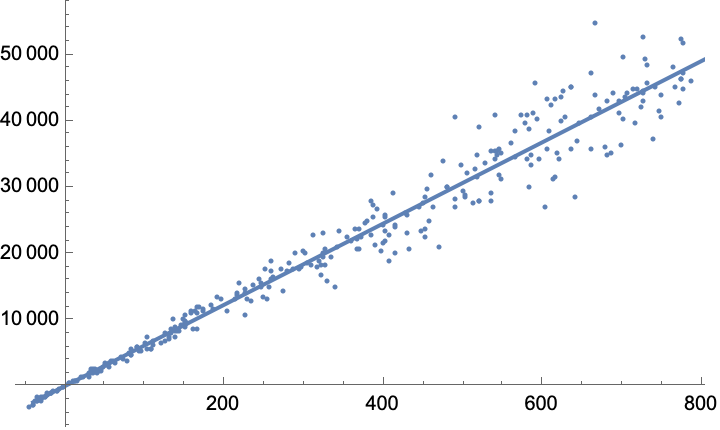
\includegraphics[width=0.9\textwidth]{reg4.png}
	   \caption*{(a)}
	\end{minipage}\hfill
	\begin{minipage}{0.45\textwidth}
	   \centering
	   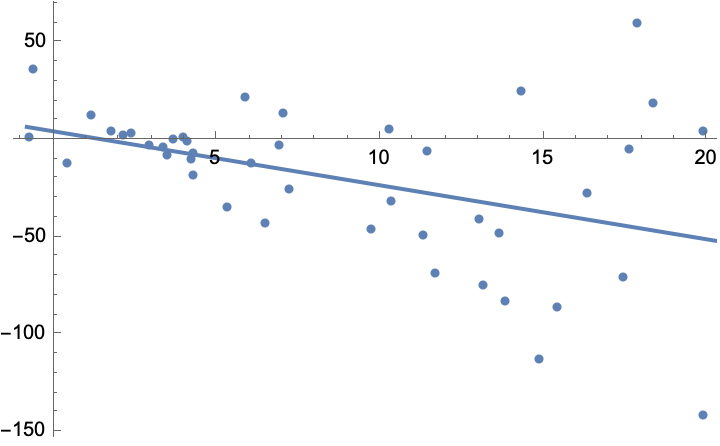
\includegraphics[width=0.9\textwidth]{reg1.png}
	   \caption*{(b)}
	\end{minipage}
	\begin{minipage}{0.45\textwidth}
	   \centering
	   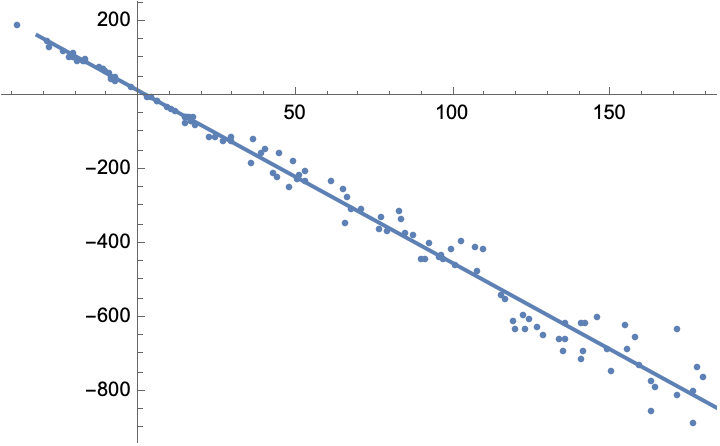
\includegraphics[width=0.9\textwidth]{reg2.png}
	   \caption*{(c)}
	\end{minipage}
	\begin{minipage}{0.45\textwidth}
	   \centering
	   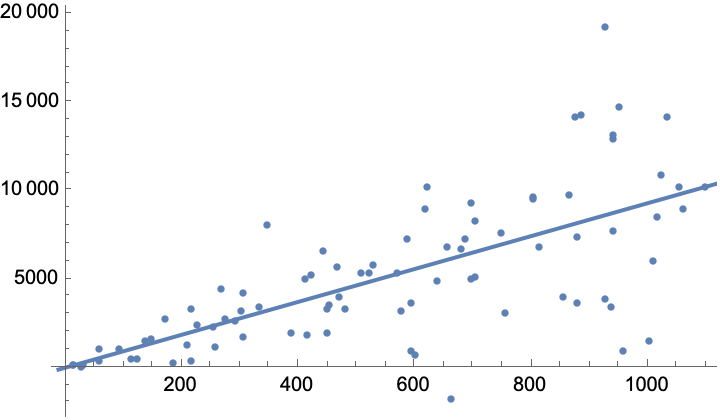
\includegraphics[width=0.9\textwidth]{reg3.png}
	   \caption*{(d)}
	\end{minipage}
	\end{figure}

\begin{enumerate}[(i)]
\item \usol{0.5cm}{}: $R= 0.981608$
\item \usol{0.5cm}{}: $R= 0.693245$
\item \usol{0.5cm}{}: $R= -0.425885$
\item\usol{0.5cm}{}: $R= -0.991438$
\end{enumerate} 


\end{document}